\chapter{Поглощение света многослойной наночастицей} \label{chapt4}
\underline{\textbf{В четвёртой главе}} рассматривается явление
поглощения света многослойной наночастицей.

Достоинством теории Ми является используемое разложение поля по
сферическим векторным гармоникам, что позволяет разделить вклад в
общее поле от электрического и магнитного дипольного резонанса, а
также вклад резонансов квадруполей и мультиполей более высокого
порядка. Таким образом, становится возможен покомпонентный анализ
спектрального отклика многослойной сферы в зависимости от её
дизайна. Например, в ряде случаев удаётся совместить в спектре
рассеяния положение нескольких резонансов (например, электрических
дипольного и квадрупольного), что создаёт эффект
суперрассеяния~\cite{Fan-2010,Fan-2011}.

В данной главе был рассмотрен аналогичный эффект суперпоглощения
для наночастицы $Si/Ag/Si$, когда сечение поглощения сферической
наночастицы превышает фундаментальный предел поглощения резонансно
возбуждённого мультиполя максимального порядка. Ранее в своей
работе~\cite{Tribelsky-2011} М.И. Трибельский показал, что существует
верхний предел, ограничивающий возможности поглощения для одного
мультиполя, коэффициенты Ми для поглощения электрическими
$\tilde{a}_n= {\rm Re}\{a_n\} - |a_n|^2 $ и магнитными
$\tilde{b}_n= {\rm Re}\{b_n\} - |b_n|^2 $ модами не могут превысить
значения $1/4$.  При совмещении нескольких резонансов становится
возможным преодолеть этот фундаментальный предел. В этом случае
сечение поглощения оказывается больше, чем у однородной частицы того
же размера из произвольного изотропного материала.

При исследовании поглощения света наночастицами исследовались
трёхслойные частицы из заранее выбранных материалов, поэтому в
качестве параметров оптимизации использовались толщины составных
слоёв.  Целью оптимизации было получение структур с максимальной
эффективностью поглощения $Q_{\rm sca} = C_{\rm abs}/\pi R^2$ для
заданной длины волны, где $C_{\rm abs}$ это сечение поглощения, а $R$
это внешний радиус наночастицы.  Результат оптимизации для различных
значений $R$ представлен на рисунках~\ref{img:q-abs}(а-в). На
рисунке~\ref{img:q-abs}(а) дополнительными пунктирными линиями
отмечены максимально достижимые эффективности поглощения для
дипольного ($n=1$) и квадрупольного ($n=2$) резонансов выраженные в
виде~\cite{Tribelsky-2011}
$$Q^{(n)}_{\rm  abs\ max}=\frac{2n+1}{2q^2}$$
через параметр размера $q=2\pi R/\lambda$.  В рассматриваемой системе
максимальный порядок резонансного возбуждения мультиполей ограничен
квадруполем ($n=2$). Так как дизайны с внешним радиусом $R>60$~нм
демонстрируют большую эффективность поглощения, то выполняются условия
для режима суперпоглощения.

\begin{figure}[t]
  \begin{minipage}[ht]{0.495\linewidth}
    \center{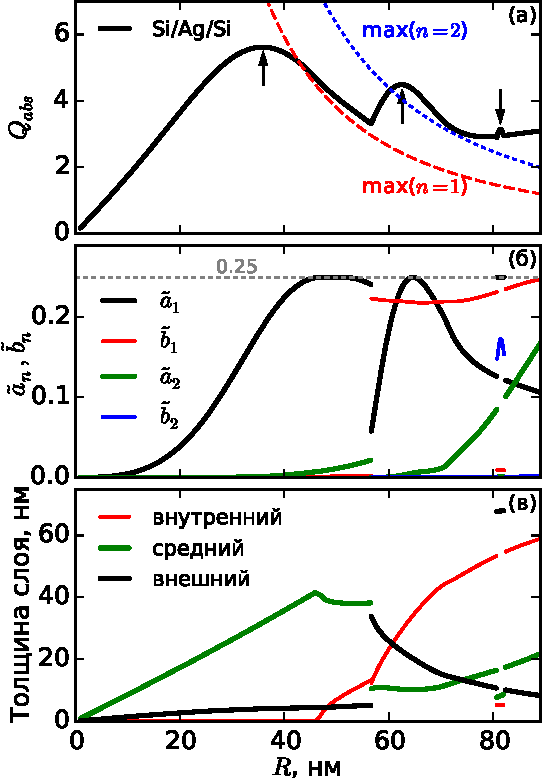
\includegraphics[height=1.35\linewidth]{2015-04-01-Qabs-SiAgSi-overview}}
  \end{minipage}
  \hfill
  \begin{minipage}[ht]{0.495\linewidth}
    \center{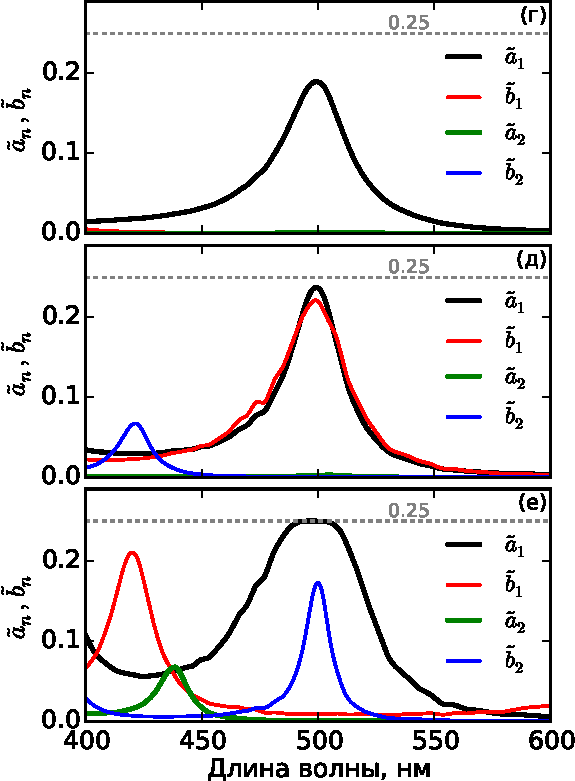
\includegraphics[height=1.35\linewidth]{2015-04-01-SiAgSi-ab-spectra4}}
  \end{minipage}
  \caption{ (а-в) Результат оптимизации эффективности поглощения
    $Si/Ag/Si$ наночастицей в зависимости от её внешнего радиуса, (а)
    эффективность поглощения, (б) коэффициенты поглощения в разложении
    Ми, где $\tilde{a}_1$ и $\tilde{a}_2$ относятся к электрическим, а
    $\tilde{b}_1$ и $\tilde{b}_2$ к магнитным диполю и квадруполю, (в)
    толщины составных слоёв наночастиц, (г-е) спектры коэффициентов
    поглощения в разложении Ми для дизайнов, соответствующих локальным
    максимумам на рисунке~\ref{img:q-abs}а.}
  \label{img:q-abs}  
\end{figure}


На рисунке~\ref{img:q-abs}(б) изображены значения коэффициентов Ми для
поглощения различными модами, горизонтальной пунктирной линией
отмечено значение теоретически достижимого предела для них, равное
1/4. В случае небольшого размера частицы основной вклад в поглощение
даёт электрический диполь $\tilde{a}_1$.  При оптимизации дизайнов для
$R > 56.6$~нм оказалось, что дизайны с поглощением одновременно на
электрическом и магнитном диполях позволяет достичь большего общего
сечения поглощения, чем в случае поглощения только электрическим
диполем. Такое качественное изменение соответствует разрывам линий на
рисунках~\ref{img:q-abs}(б-в) и реализует режим суперпоглощения.
Необходимо отметить, что для небольшого диапазона размеров частицы
$80.7<R<82.1$~нм оптимальное поглощение обеспечивает использование
электрического дипольного $\tilde{a}_1$ и магнитного квадрупольного
$\tilde{b}_2$ резонансов, что приводит ещё к двум разрывам линий на
рисунках для соответствующих значений внешнего радиуса~$R$.

На рисунке~\ref{img:q-abs}(в) представлены толщины составных слоёв
наночастицы, полученные в результате оптимизации эффективности
поглощения.  Неожиданно оказалось, что дизайны с преобладающим
дипольным механизмом поглощения (т.е. для размеров частицы менее
56.6~нм) могут быть двух видов.  Чтобы получить наилучшее поглощение
для $R<46$~нм, хватает использования всего двух слоёв, при оптимизации
толщина внутреннего слой исходного трёхслойного дизайна обратилась в
ноль.  При $R=46$~нм поглощение диполем почти достигает своего
теоретического предела ($\tilde{a}_1>0.249$), чтобы удерживать его
вблизи этого значения для больших значений $R$, оптимизатор начинает
наращивать толщину внутреннего кремниевого слоя.  В свою очередь, это
приводит к появлению слабого поглощения  $\tilde{a}_2$,
что, впрочем, не позволяет достичь режима суперпоглощения для $n=2$.

Для расчёта спектров на рисунках~\ref{img:q-abs}(г-е) были
использованы экспериментальные дисперсионные зависимости для
показателей преломления из работы\cite{palik-1997}. Спектры
коэффициентов поглощения в разложении Ми построены для дизайнов,
соответствующих локальным максимумам на
рисунке~\ref{img:q-abs}(а). Спектр для дизайна с внешним радиусом
$R=36$~нм на рисунке~\ref{img:q-abs}(г) подтверждает дипольный
характер поглощения с резонансом на выбранной для оптимизации длины
волны $\lambda=500$~нм.  Спектры дизайнов с максимумами поглощения для
$R=63$~нм и $R=81$~нм (рисунки~\ref{img:q-abs}(д) и~\ref{img:q-abs}(е)
соответственно) обладают типичной для суперпоглощения структурой с
вырождением нескольких резонансов. На этих спектрах присутствуют
дополнительные резонансы, которые, впрочем, расположены в значительном
отдалении от выбранной для оптимизации длины волны, поэтому их вклад в
общее поглощение мал.

Особо надо отметить, что для получения максимальной эффективности
поглощения вовсе не требуется режим суперпоглощения.  Из
рисунка~\ref{img:q-abs}(а) следует, что максимальная эффективность
соответствует малым размерам частицы, где значение коэффициента Ми для
поглощения заметно меньше теоретического предела.  Среди всех
рассмотренных структур двухслойная частица $Ag/Si$ с внешним радиусом
36~нм обладает максимальной эффективностью поглощения.  Для неё
сечение поглощения более чем 5 раз превысило её геометрическое
сечение. Дополнительным преимуществом таких частиц может являться то,
что они должны быть проще и дешевле в производстве по сравнению с
трёхслойными.  В то же время для частиц большего размера ($R>60$~нм
для рассмотренных материалов) максимальная эффективность получается в
режиме суперпоглощения.  Это может оказаться существенно для случая,
когда изготовление многослойных частиц меньшего размера не доступно по
какой-либо технологической причине.

\clearpage